\subsection{Part A: Docking simulation}

\subsubsection{Simulation environment}
\label{sec:method-sim}

The simulation runs on ROS~2 Jazzy with Gazebo (gz-sim~8, DART physics) and a battle-tested ArduSub autopilot with ArduPilot Gazebo plugin. The BlueROV2 Heavy vehicle model, its hydrodynamic and buoyancy plugins, and the simulation bring-up derive from the open-source Blue framework \cite{blue2024software,palmer2024angler}, of which this project maintains a git fork adapted to ROS~2 Jazzy. The simulate BlueROV2 has a forward camera at 10~Hz. The world places a docking station 5~m  ahead of the vehicle spawn at 1.5~m depth, with all nine ArUco markers (47.5~mm to 200~mm).

\begin{figure}[H]
    \centering
    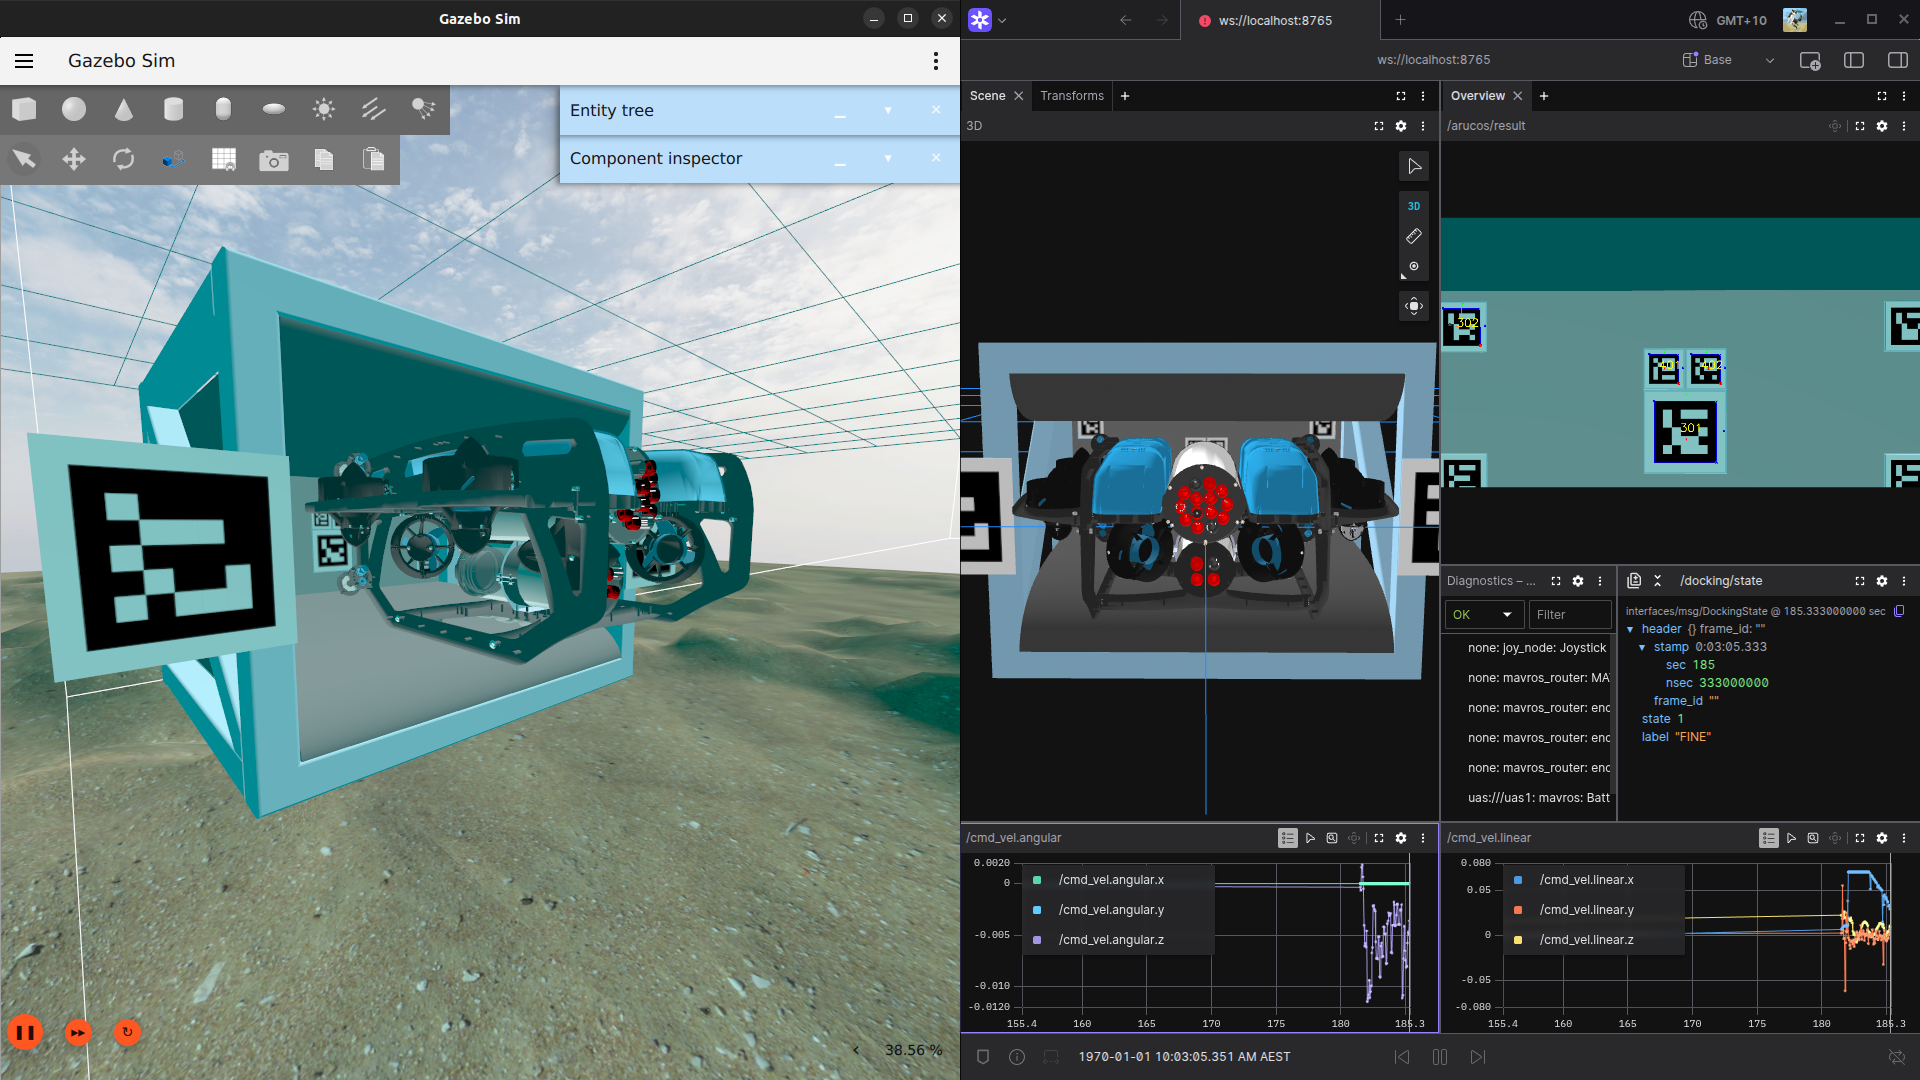
\includegraphics[width=0.85\textwidth]{Figures/simulation_gazeboxfoxglove.png}
    \caption{The simulation environment during a docking trial, with the Gazebo world
        view (left) and live telemetry in Foxglove (right) showing the onboard
        camera stream, ArUco detections and the docking state machine state.}
    \label{fig:sim-env}
\end{figure}

Dock swaying motion is generated by a custom Gazebo plugin that drives the dock through a sinusoidal sway and heave of amplitude of 0.1~m with 90-degree relative phase, producing an orbital motion representative of wave-driven forces on the moored structure. Mechanical capture and contact are not modelled such that success is defined at the capture envelope (Section~\ref{sec:method-experiment}) and potential dock contacts are post-processed during data analysis.

The swept period band and amplitude are mapped from the real wave forcing in New South Wales. The wave energy occupies roughly 5 to 20~s, and the mean sea state off the NSW coast is a wave height of 1.6~m at an 8~s period, in context of the operation of this work \cite{holthuijsen2007waves, short1992wave, kinsela2024nearshore}. The dock is forced by the wave orbital motion, whose amplitude decays with depth exponentially as $e^{-kz}$, with $k = 2\pi/L$ and deep-water wavelength $L = gT^2/2\pi \approx 1.56\,T^2$ \cite{holthuijsen2007waves}. As a result, the simulated 0.1~m amplitude corresponds, in the mean NSW sea state, to dock at approximately 19~m depth for the 6~s period, 33~m at 8~s, 52~m at 10~s and more than 200~m at 20~s. Therefore, sweeping 6 to 20~s at a fixed 0.1~m amplitude isolates the period dependence while keeping every trial identifiable with a physically realistic sea state in NSW and operating depth.

\subsubsection{Marker layout}
\label{sec:method-layout}

Each marker on the dock are sized and categorised by their function. The two largest markers (200~m class) sit on the outer front edge of the structure, where they subtend the pixels needed for long-range acquisition. The mid-sized and small markers populate the dock interior. The two smallest (IDs 401 and 402) are placed at the height of the vehicle's camera in the docked position, so that markers remain in frame during the final phase of docking. This follows the fractal marker principle, in which markers of several sizes are combined so that pose estimation survives across the full range span \cite{romeroramirez2019fractal}, though the markers are distributed spatially instead of nested. The dock structure itself was kept deliberately minimal, and its mechanical design is not a subject of this thesis. The marker IDs are likewise arbitrary with respect to detection, since they were assigned so that the leading digit encodes the size class (2xx outer, 3xx interior, 4xx eye level), which is a naming convention to ease debugging, and each ID merely selects a stock pattern from the dictionary with the least black and white pixel ratio. Optimising the bit patterns themselves for detectability at longer range is not considered in this thesis.


\begin{figure}[H]
    \centering
    \begin{tikzpicture}
  \node[anchor=south west, inner sep=0] (img) {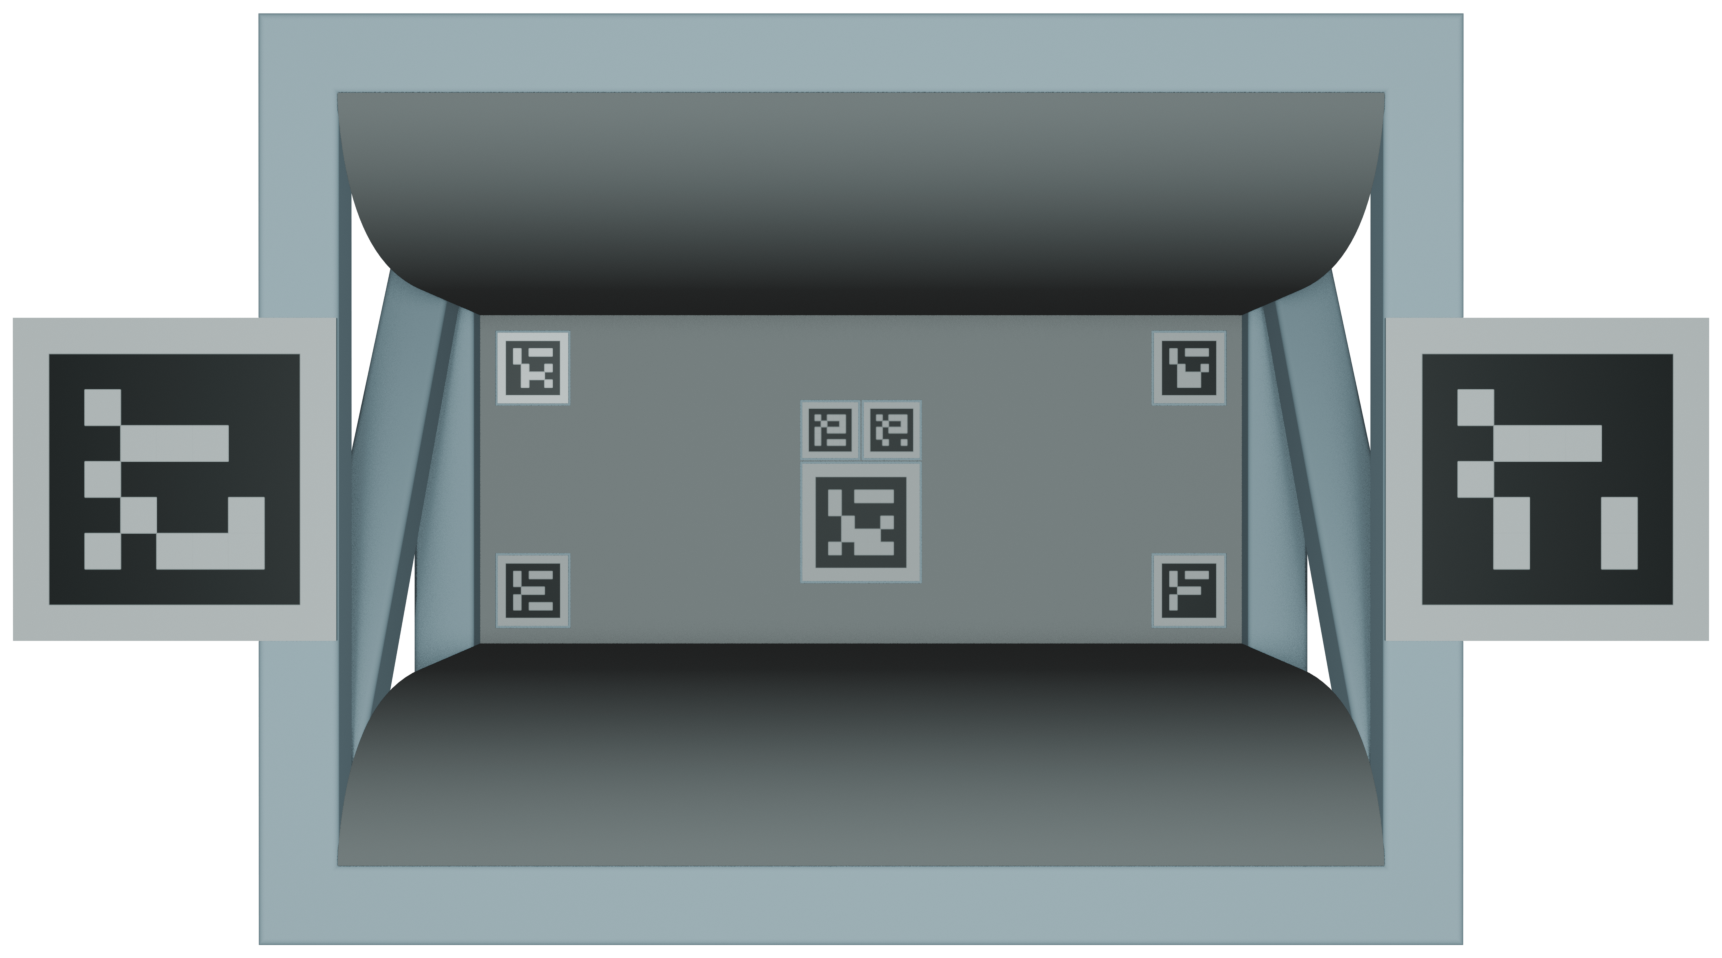
\includegraphics[width=0.8\textwidth]{Images/dock_front_view.png}};
  \begin{scope}[x={(img.south east)}, y={(img.north west)},
      lab/.style={font=\scriptsize\bfseries, text=white, fill=black, fill opacity=0.55,
                  text opacity=1, inner sep=2pt, rounded corners=1pt},
      arr/.style={orange, thick, -{Stealth[length=1.6mm]}}]
    \node[lab] (l201) at (0.075,0.160) {201};
    \draw[arr] (l201) -- (0.095,0.425);
    \node[lab] (l202) at (0.925,0.160) {202};
    \draw[arr] (l202) -- (0.904,0.425);
    \node[lab] (l301) at (0.565,0.240) {301};
    \draw[arr] (l301) -- (0.514,0.408);
    \node[lab] (l302) at (0.245,0.760) {302};
    \draw[arr] (l302) -- (0.295,0.648);
    \node[lab] (l303) at (0.755,0.760) {303};
    \draw[arr] (l303) -- (0.704,0.648);
    \node[lab] (l304) at (0.755,0.240) {304};
    \draw[arr] (l304) -- (0.704,0.352);
    \node[lab] (l305) at (0.245,0.240) {305};
    \draw[arr] (l305) -- (0.295,0.352);
    \node[lab] (l401) at (0.400,0.720) {401};
    \draw[arr] (l401) -- (0.464,0.588);
    \node[lab] (l402) at (0.600,0.720) {402};
    \draw[arr] (l402) -- (0.536,0.588);
  \end{scope}
\end{tikzpicture}

    \caption{Dock front view showing the size-graded marker placement, with the
        200~mm class (201, 202) on the outer edge, mid and small markers
        (301 to 305) in the interior, the smallest pair (401, 402) at camera
        eye level in the docked position.}
    \label{fig:dock-layout}
\end{figure}

\subsubsection{Perception (simulated ArUco pipeline)}

The full perception pipeline runs in the loop such that the ground truth is filtered out for the controller. Markers are detected on the simulated forward camera and each markers detected is then converted to a derived dock-origin pose using the known marker layout and orientation. A spatial-consensus test rejects outlier detections while surviving markers are fused by inverse-variance weighting with a range noise model ($\sigma = \alpha r^2 / s$ for a marker of size $s$ at range $r$) so this makes distant and small markers contribute less than larger ones.

The fused measurement feeds a nine-state error-state Kalman filter. The state holds the dock position, the dock velocity, and a small rotation correction. Rather than filtering the orientation quaternion directly, the filter tracks a small-angle error relative to a reference quaternion and folds it back into the reference after each update \cite{sola2017quaternion}.

The fused measurement then feeds a nine state Kalman filter. The state includes the dock position, the dock velocity, and a small rotation correction. Instead of filtering the orientation quaternion directly, the filter tracks a small angle error relative to a reference quaternion and folds it back into the reference per update \cite{sola2017quaternion}. Two process-noise regimes are also defined. The \emph{static} regime assumes zero initial velocity uncertainty and zero velocity process noise, which is algebraically equivalent to a constant-position filter. The \emph{sway} regime incorporates the velocity state with acceleration as white noise of density $\sigma_a$ (0.16~m/s$^2$ nominal, exposed as a parameter), allowing dock velocity estimation and the feedforward of Section~\ref{sec:method-control}. Each update is gated by a Mahalanobis gate, while the velocity state is bounded by a physical dock-speed limit (0.2~m/s).

\begin{figure}[H]
    \centering
    \begin{tikzpicture}[font=\scriptsize, >={Stealth[length=2mm]},
  box/.style={draw, rounded corners=1pt, align=center, minimum height=9mm, inner sep=3pt}]
  \node[box] (meas) {fused\\measurement};
  \node[box, right=7mm of meas] (gate) {Mahalanobis\\gate};
  \node[box, right=7mm of gate] (upd) {update\\ $[\,\delta p \;\; \delta v \;\; \delta\theta\,]$};
  \node[box, right=7mm of upd] (bound) {bounds:\\ $|v| \leq 0.2$ m/s,\\ $\sigma_p$ ceiling};
  \node[box, right=7mm of bound] (out) {pose, twist,\\health};
  \node[box, below=7mm of upd] (pred) {predict (30 Hz)\\ \emph{static}: $v$ pinned $\;|\;$ \emph{sway}: WNA $\sigma_a$};
  \draw[->] (meas) -- (gate);
  \draw[->] (gate) -- (upd);
  \draw[->] (upd) -- (bound);
  \draw[->] (bound) -- (out);
  \draw[->] (pred) -- (upd);
\end{tikzpicture}

    \caption{Filter structure, showing the nine-state error-state filter with the two
        process-noise regimes, the measurement gate and the state bounds.}
    \label{fig:kf}
\end{figure}

\subsubsection{Guidance and control}
\label{sec:method-control}

In the coarse approach phase, the vehicle approaches the standoff point 1~m out along the dock entry axis via per-axis proportional-derivative (PD) control, while a distance-gated surge cap bounds the closing speed (the speed limit reduces as the vehicle gets closer). At the point of handoff (transitioning to the fine alignment phase), the transition is gated by three tolerances, namely position, boresight offset and yaw. In addition, the vehicle must be moving with the standoff point, not merely crossing it. Its velocity relative to the point must stay below 0.15~m/s, obtained by differentiating the vehicle-to-standoff position error over time, with exponential smoothing to suppress the noise that differentiation amplifies. All conditions must hold through a debounce window before the handoff latches. This guards against a false handoff at a sway zero crossing, where the position error is momentarily small while the dock is moving at its fastest. Note that this phase runs with ArduPilot's \textsc{depth\_hold} flight mode, which provides automatic depth keeping from the pressure sensor and attitude stabilisation on roll and pitch. The coarse controller therefore only commands surge, sway and yaw, while the autopilot holds the vehicle level and at depth.

Fine alignment implements align-then-advance, where surge toward the entry is inhibited until lateral, vertical and yaw errors are within alignment tolerances, with the autopilot in stabilise mode so the controller owns depth. The seat criterion (definition of docked) is a debounced 0.10~m range to the entry with 0.03~m lateral and vertical tolerances. The 0.10~m value is derived from the measured sensing envelope in Section~\ref{sec:results-a}, which shows marker visibility collapsing below approximately 5~cm, so the seat is confirmed where vision is still reliable and the final centimetres are delegated to the capture mechanism assumed by the envelope definition.

In the fine alignment phase, the vehicle follows an align-then-advance strategy.
Only until the lateral, vertical and yaw errors are all within their alignment tolerances, so the vehicle first centres itself on the entry axis and then advances forward with surge. The seat criterion (the definition of docked) is a debounced range of 0.10~m to the entry, with 0.03~m lateral and vertical tolerances. The 0.10~m value is derived from the measured sensing envelope in Section~\ref{sec:results-a}, which shows marker visibility collapsing below approximately 5~cm. Therefore, the seat is confirmed while vision is still reliable, and the final centimetres are delegated to the capture mechanism, which is out of scope. Note that this phase runs with ArduPilot's \textsc{stabilise} flight mode instead of \textsc{depth\_hold}.he fine controller therefore owns the depth axis as well, since the vehicle must track the vertical motion of the swaying entry axis rather than hold a fixed depth.

Both the coarse and fine controllers accept a dock-velocity feedforward, which is built from the filter's velocity state rotated into the body frame. Three mechanisms shape this feedforward:
\begin{enumerate}
    \item Feedforward velocity clamped separately at 0.25~m/s.
    \item Scaled by a distance-gated ramp, which is zero beyond 1.5~m from the standoff point and full when within 0.3~m.
    \item The velocity is converted to command units (the units to be fed into the ArduPilot controller) by a gain of 0.6, since the command channel is effort-like rather than velocity-like (a measured steady gain of 1.3 to 1.6) and approximately 240~ms of lag between command and vehicle velocity, which is further discussed in the failure analysis of Section~\ref{sec:results-a}.
\end{enumerate}
\noindent In the \emph{static} filter regime, the velocity estimate is set to zero, so no feedforward in the system.

\begin{figure}[H]
    \centering
    \begin{tikzpicture}[font=\scriptsize, >={Stealth[length=2mm]}, scale=1.15]
  % dock cage (top view), entry faces left
  \fill[fill={white!70!blue}] (8.0,-0.75) rectangle (9.6,0.75);
  \fill[white] (8.0,-0.55) rectangle (9.4,0.55);
  \draw[thick] (8.0,-0.75) rectangle (9.6,0.75);
  \draw[thick] (8.0,-0.55) rectangle (9.4,0.55);
  \node at (8.8,1.05) {dock (top view)};
  % entry axis
  \draw[dashed] (0.2,0) -- (8.0,0);
  \node at (5.2,0.25) {\tiny entry axis};
  % blackout zone
  \fill[red!12] (7.6,-0.6) rectangle (8.0,0.6);
  \node[red!60!black, align=center] at (6.3,-1.45) {\tiny vision blackout $<$ 0.05 m};
  \draw[red!60!black, ->] (6.7,-1.3) -- (7.8,-0.5);
  % entry plane + aperture
  \draw[<->] (8.1,-0.55) -- (8.1,0.55);
  \node[align=center] at (9.3,-1.15) {\tiny aperture\\ \tiny $\pm$0.15 m};
  \draw[->] (9.0,-0.98) -- (8.15,-0.4);
  % seat point
  \draw[thick] (7.2,-0.15) -- (7.2,0.15);
  \node[align=center] at (6.1,0.95) {\tiny seat: 0.10 m,\\ \tiny $\pm$0.03 m lateral};
  \draw[->] (6.4,0.72) -- (7.15,0.2);
  % standoff
  \node at (3.4,0) {$\times$};
  \node[align=center] at (3.4,0.55) {\tiny standoff point\\ \tiny (coarse target)};
  % vehicle (side-view render, front faces the dock)
  \node[inner sep=0] (rov) at (1.4,0) {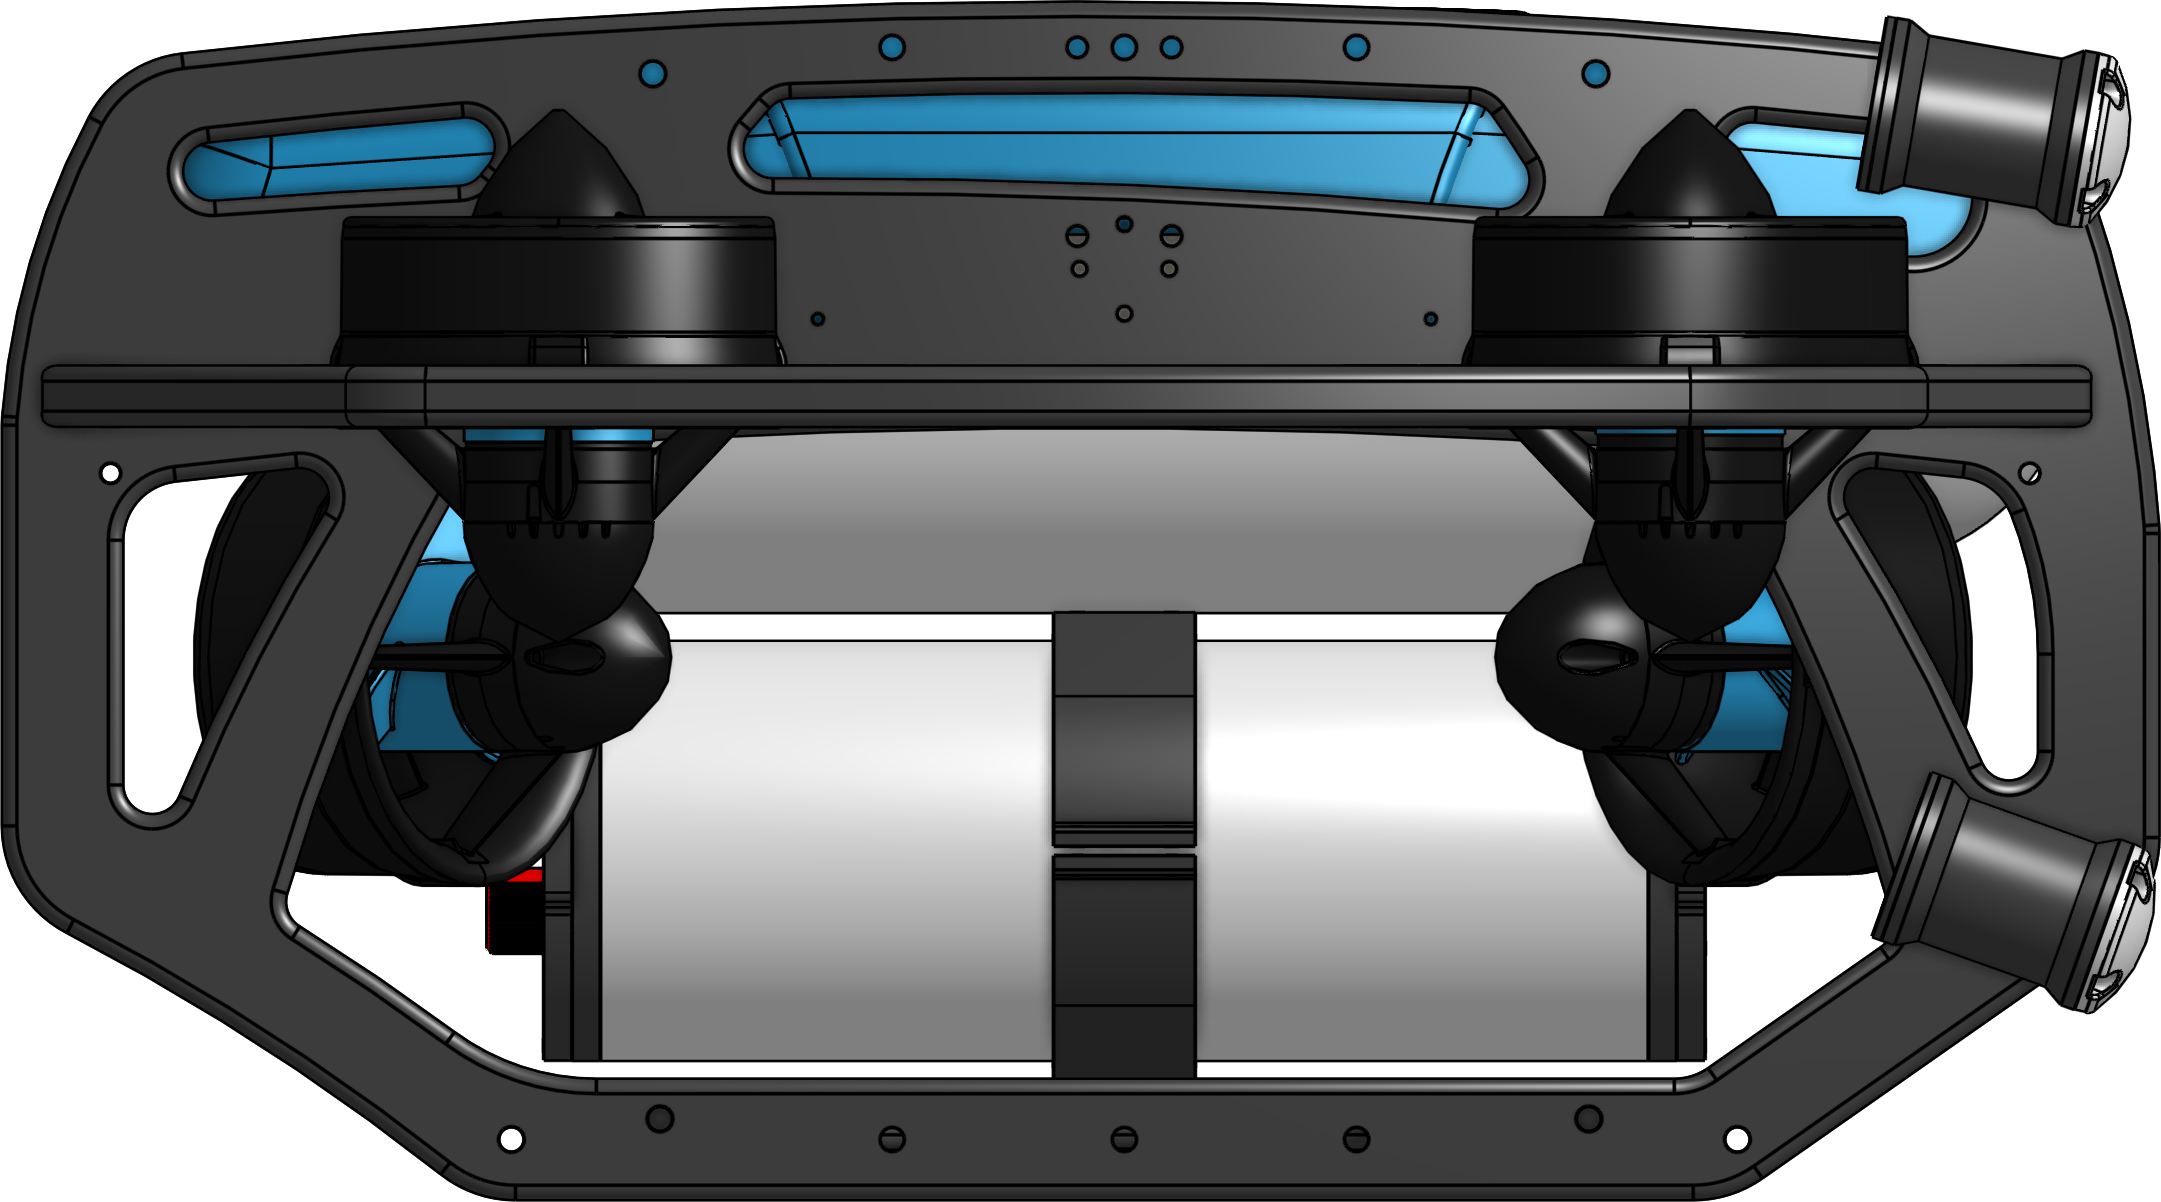
\includegraphics[width=18mm]{Images/BROV2_heavy_side.png}};
  \node at (1.4,-0.75) {\tiny ROV};
  \draw[->] (rov.east) ++(1mm,0) -- (3.15,0);
  % distance annotations
  \draw[|<->|] (3.4,-0.9) -- (8.0,-0.9);
  \node at (5.0,-1.1) {\tiny 1.0 m (not to scale)};
\end{tikzpicture}

    \caption{Terminal docking geometry (top view, not to scale), showing the coarse
        standoff point, the entry axis, the 0.15~m scoring aperture, the
        0.10~m seat criterion and the close-range vision blackout.}
    \label{fig:geometry}
\end{figure}

\subsubsection{Experimental method}
\label{sec:method-experiment}

The envelope experiment sweeps filter regime (\emph{static} vs \emph{sway}) by dock sway period $\{20, 16, 12, 10, 8, 6\}$~s with three sway start phases per cell ($n{=}3$), 38 trials per sweep. Each trial receives one of three outcomes:
\begin{enumerate}
    \item \textsc{clean dock}: docked with no pre-latch off-aperture crossing.
    \item \textsc{contact}: the vehicle clipped through the dock structure outside
          the 0.15~m entry aperture before seating (contact is not physically
          modelled, so the overlap is detected in scoring). The trial is censored
          from that instant.
    \item \textsc{no dock}: the vehicle has been timed out.
\end{enumerate}
The sweep was run twice, on two hosts (real-time factors 0.6 and 1.0) and two filter revisions, to ensure that the trial result do not depend on load, hardware or incidental tuning.

\begin{table}[H]
    \centering
    \caption{Trial parameters of the docking envelope sweep.}
    \label{tab:sweep-params}
    \begin{tabular}{l l}
        \hline
        Parameter                & Values                                                  \\
        \hline
        Filter regime            & \emph{static} (baseline), \emph{sway} (method)          \\
        Dock sway period         & $\{20, 16, 12, 10, 8, 6\}$~s                            \\
        Sway start phase         & $\{0,\ 2\pi/3,\ 4\pi/3\}$~rad ($n{=}3$ per cell)        \\
        Sway and heave amplitude & 0.1~m each, $90^\circ$ relative phase (orbital)         \\
        Static-dock sanity cell  & one per regime                                          \\
        Trials per sweep         & 38                                                      \\
        Sweep repetitions        & 2 (real-time factors 0.6 and 1.0, two filter revisions) \\
        Total trials             & 76                                                      \\
        \hline
    \end{tabular}
\end{table}


